\documentclass[a4paper,12pt]{article}
\usepackage[utf8]{inputenc}
\usepackage[polish]{babel}
\usepackage[T1]{fontenc}
\usepackage{geometry}
\usepackage{graphicx}
\usepackage{enumitem}
\usepackage{hyperref}
\usepackage{longtable}
\geometry{margin=2.5cm}

\title{Sprawozdanie z realizacji projektu - Język Java}
\author{Markiian Novytskyi, Arseni Fayeu}
\date{\today}

\begin{document}

\maketitle

\section*{1. Tytuł projektu}
\textbf{Java Royale: Multiplayer Top-Down Battle Royale Shooter}\\
\textit{Wieloosobowa gra akcji typu battle royale z widokiem z góry. Architektura klient--serwer z autorytatywnym serwerem gry, klientem graficznym libGDX oraz warstwą sieciową Netty (TCP dla lobby, UDP dla rozgrywki).}

\section*{2. Założone vs. zrealizowane funkcjonalności}

\begin{longtable}{|p{6cm}|p{4cm}|p{4cm}|}
\hline
\textbf{Funkcjonalność} & \textbf{Założona} & \textbf{Zrealizowana} \\
\hline
System lobby (połączenie, roster, ready, countdown) & Tak & Tak \\
\hline
Mechanika ruchu (WSAD + predykcja klienta) & Tak & Tak \\
\hline
System walki (strzelanie, trafienia, eliminacja) & Tak & Tak \\
\hline
Synchronizacja świata (snapshots UDP) & Tak & Tak \\
\hline
Mechanika strefy (storm, obrażenia poza strefą) & Tak & Tak \\
\hline
Warunki zwycięstwa (match end, statystyki) & Tak & Tak \\
\hline
Skalowalność do 25--50 graczy (architektura) & Tak & Częściowo \\
\hline
Testy obciążeniowe wielu klientów & Tak & Nie \\
\hline
\end{longtable}

\textbf{Zrealizowano: 6 z 7 zaplanowanych funkcjonalności (86\%)}

\section*{3. Realizacja wymagań}

\subsection*{Funkcjonalne vs. niefunkcjonalne}

\begin{longtable}{|p{6cm}|p{4cm}|p{4cm}|}
\hline
\textbf{Typ Wymagań} & \textbf{Założone} & \textbf{Zrealizowane} \\
\hline
Funkcjonalne & 7 & 6 \\
\hline
Niefunkcjonalne & 5 & 4 \\
\hline
\end{longtable}

\textbf{Procent realizacji:} Funkcjonalne: 86\%, Niefunkcjonalne: 80\%

\subsection*{Odchylenie od specyfikacji początkowej}
W pierwotnej specyfikacji cała komunikacja sieciowa opisana była jako TCP.
W implementacji zastosowano model hybrydowy:
\begin{itemize}
    \item \textbf{TCP (port 25565)} --- lobby: handshake, roster, matchmaking, countdown, koniec meczu.
    \item \textbf{UDP (port 25566)} --- rozgrywka: input gracza, snapshots świata, strefa, przedmioty.
\end{itemize}
Uzasadnienie: niskie opóźnienia i wysoka częstotliwość pakietów w fazie gry; zdarzenia krytyczne (śmierć, koniec meczu) nadal przesyłane przez TCP.

\subsection*{Wymagania niefunkcjonalne}
\begin{itemize}
    \item \textbf{Wydajność (60 FPS)} --- Tak (libGDX, płynna rozgrywka dla wielu klientów testowych).
    \item \textbf{Skalowalność (25--50 graczy)} --- Częściowo (architektura tick-based; testy głównie dla 2--4 graczy).
    \item \textbf{Niskie opóźnienia} --- Tak (UDP dla gameplay, predykcja i rekonsyliacja po stronie klienta).
    \item \textbf{Stabilność} --- Częściowo (obsługa rozłączeń, walidacja seq; brak reconnect w trakcie meczu).
    \item \textbf{Modularność Maven} --- Tak (moduły \texttt{common}, \texttt{networking}, \texttt{app}).
\end{itemize}

\section*{4. Rzeczywisty nakład pracy}

\begin{itemize}
    \item Planowany czas pracy: 155 godzin
    \item Rzeczywisty czas pracy: 155 godzin
\end{itemize}

Rozbicie (zgodnie ze specyfikacją):
\begin{itemize}
    \item Architektura i Maven: 10 h
    \item Networking (Netty TCP/UDP): 30 h
    \item Rendering (libGDX): 45 h
    \item Logika gry (kolizje, strefa, strzelanie): 30 h
    \item UI / HUD: 15 h
    \item Testowanie i debugging: 25 h
\end{itemize}

\section*{5. Napotkane problemy i rozwiązania}

\begin{itemize}
    \item \textbf{Regresja dekodowania rosteru TCP:} częściowe ramki TCP powodowały pustą listę graczy w lobby.\\
    \textit{Rozwiązanie:} test regresyjny \texttt{TcpFromServerDecoderRosterTest} oraz bezpieczne parsowanie w \texttt{TcpFromServerDecoder}.

    \item \textbf{ClassNotFoundException przy uruchomieniu serwera:} brak kompilacji przed \texttt{mvn exec:java}.\\
    \textit{Rozwiązanie:} \texttt{mvn clean install} przed startem serwera/klienta.

    \item \textbf{Odchylenie TCP vs UDP:} specyfikacja zakładała TCP; gameplay wymaga niższych lagów.\\
    \textit{Rozwiązanie:} hybryda TCP (lobby) + UDP (gra), opisana w \texttt{networc\_structure.md}.

    \item \textbf{Synchronizacja pozycji:} przeskoki przy opóźnieniu sieci.\\
    \textit{Rozwiązanie:} predykcja po stronie klienta, autorytatywna symulacja serwera (\texttt{MatchRuntime}), interpolacja (LERP) dla innych graczy.

    \item \textbf{Testy jednostkowe warstwy sieciowej:} niskie pokrycie na początku fazy testów.\\
    \textit{Rozwiązanie:} rozszerzenie testów JUnit 5 dla \texttt{Wire}, \texttt{UdpHeader}, dekoderów TCP oraz logiki UDP (\texttt{MatchRuntime}, \texttt{ZoneManager}, \texttt{WorldSnapshotCodec}).
\end{itemize}

\section*{6. Możliwości Rozwoju}

\begin{itemize}
    \item Delta compression snapshotów i interest management (mniej ruchu przy 25+ graczach).
    \item Reconnect w trakcie meczu (zachowanie stanu po rozłączeniu TCP).
    \item Testy obciążeniowe (stress test wielu klientów na jednej maszynie).
    \item Integracja JaCoCo w CI dla raportu pokrycia kodu.
    \item Tryb drużynowy, czat głosowy / tekstowy.
\end{itemize}

\section*{7. Zrzuty Ekranu}
\textit{Poniżej zamieszczono zrzuty ekranu aplikacji Java Royale.}

\begin{figure}[h!]
    \centering
    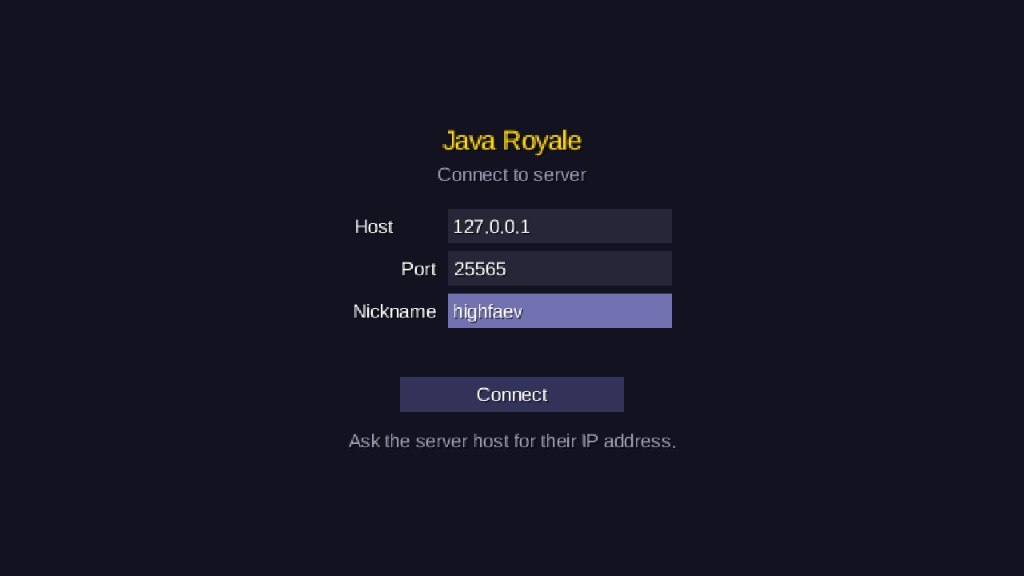
\includegraphics[width=0.9\textwidth]{screenshots/connect.png}
    \caption{Ekran połączenia z serwerem (host, port, nickname)}
\end{figure}

\begin{figure}[h!]
    \centering
    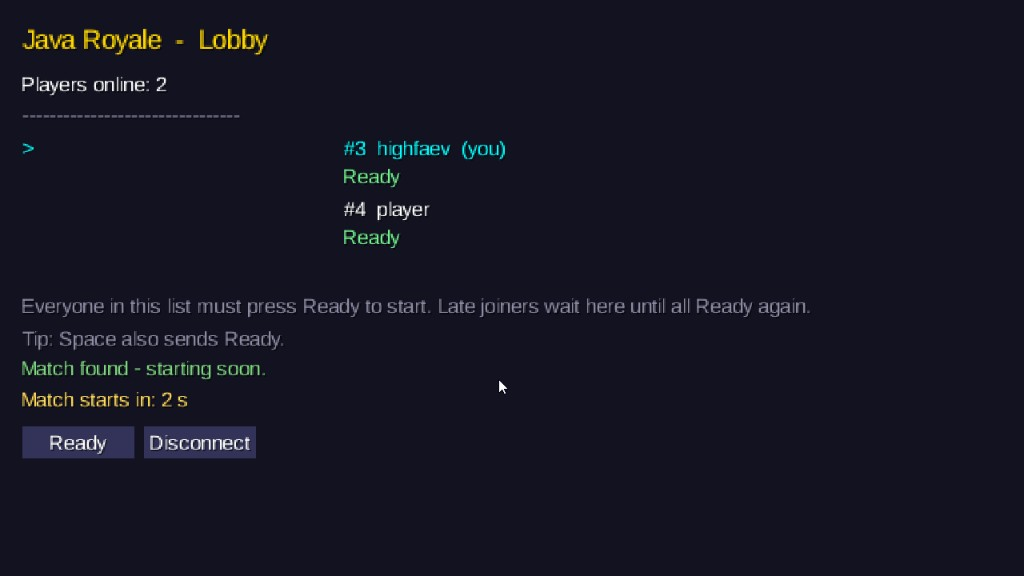
\includegraphics[width=0.9\textwidth]{screenshots/lobby.png}
    \caption{Lobby --- lista graczy, status Ready, odliczanie do startu meczu}
\end{figure}

\begin{figure}[h!]
    \centering
    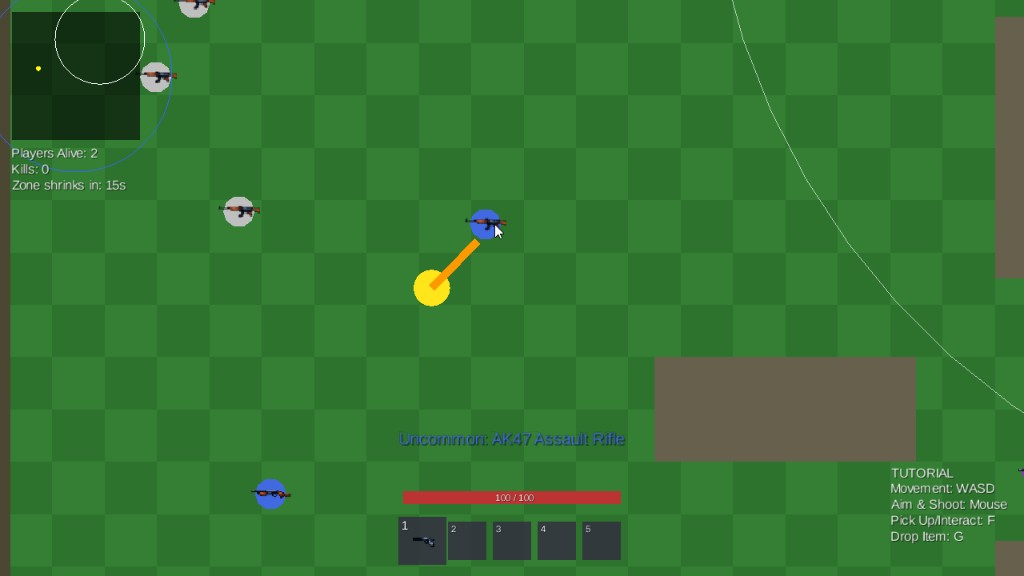
\includegraphics[width=0.9\textwidth]{screenshots/gameplay.png}
    \caption{Rozgrywka --- HUD, strefa, broń i przedmioty na mapie}
\end{figure}

\begin{figure}[h!]
    \centering
    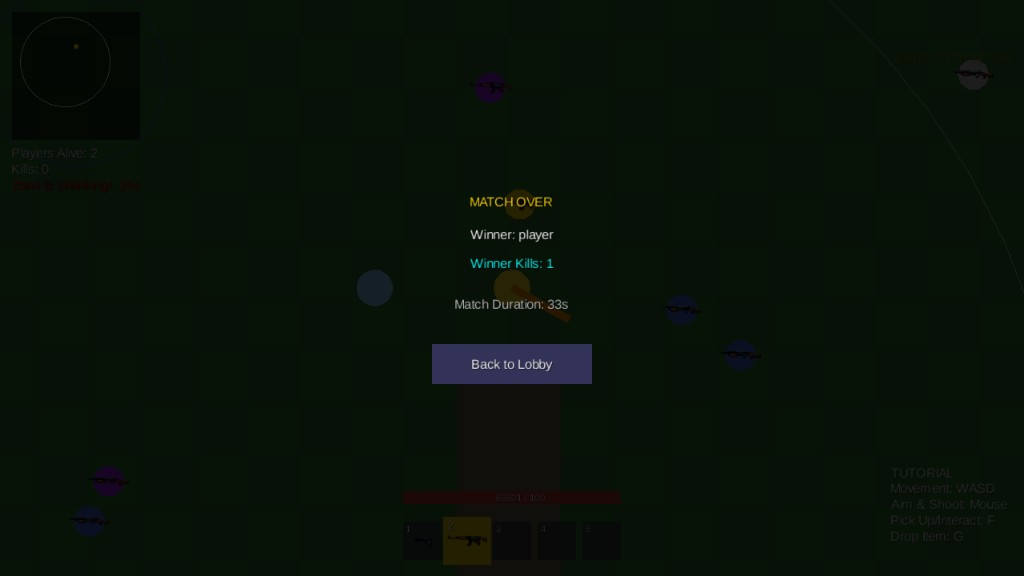
\includegraphics[width=0.9\textwidth]{screenshots/match_over.png}
    \caption{Ekran końca meczu --- zwycięzca, statystyki, powrót do lobby}
\end{figure}

\end{document}
